All model comparisons used $a = 0.263 \spbox{and} \xi =2$, while changing $b$. The non-dimensional
variable$b$was varied over $a$, because ``Henry's solution is very sensitive to changes in $b$''
(S\'egol 1994). The first comparison ( \textbf{Figure \ref{fig:b10-1}}) was done for $b=0.1$. As one
can see the contours obtained by Henry's Method are not very smooth, and may be the reason why model
comparisons using this method were unable to obtain a close match.  However, a close match for the
0.5 isochlor is seen between Newton's Method and SUTRA. For the 0.9 isochlor, Newton's Method and
SUTRA contours are almost indistinguishable. As one proceeds from the 0.9 isochlor to the 0.1
isochlor the contours of Newton's Method and SUTRA become further and further apart. This seems to
be caused by the instabilities in the upper 20\% of the solution domain for Newton's Method. These
instabilities were also seen by S\'egol \cite{Segol}, when using Henry's Method, so it appears that
this is an inherent trait in Henry's problem. However, these instabilities seem to be reduced by
increasing the total number of Fourier coefficients. It therefore may be possible to eliminate such
instabilities with a greater number of Fourier coefficients, but due to time constraints a maximum
of 1860 Fourier coefficients were used.

\begin{figure}[htp] \centering
    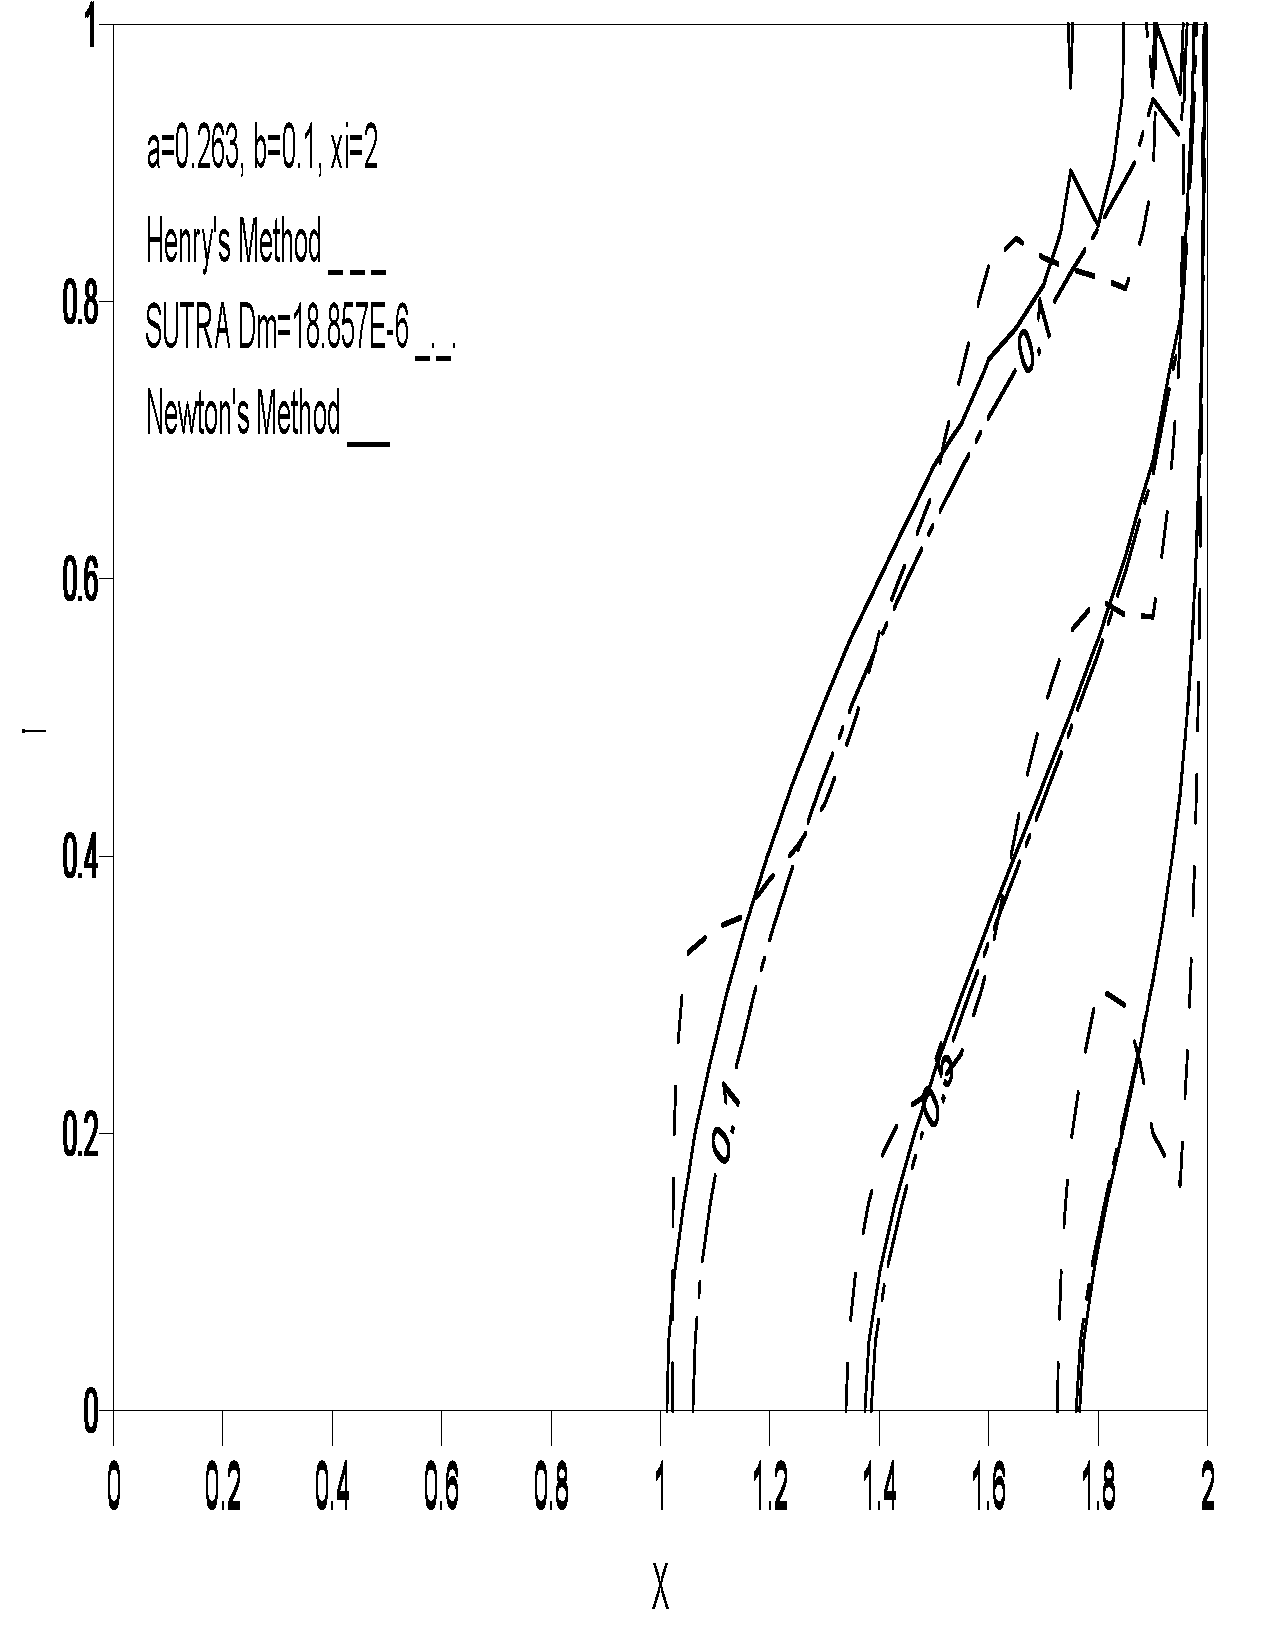
\includegraphics[totalheight=0.45 \textheight,viewport=3mm 4mm 205mm 292mm]
    {image2}
    \caption{Isochlor concentrations for $a = 0.263 \spbox{and} b =
    0.1$} \label{fig:b10-1}
\end{figure}

The second comparison ( \textbf{Figure \ref{fig:b5x10-2}}) used a value of 0.05 for $b$, and as one
can see an increase in instabilities in the upper 20\% of the solution domain resulted. As for
Henry's Method, instabilities were so great that the 0.1 isochlor contour shows up near $x=0.2
\text{ m} $. Once again the 0.9 isochlor contours for Newton's Method and SUTRA match very well, and
so does the 0.5 isochlors, but the 0.1 isochlor contours differ by a noticeable amount in their
position. Again it appears that as the concentration decreases from 0.9 to 0.1 the isochlor contours
begin to differ by greater amounts. As one can see from \textbf{Figure \ref{fig:b5x10-5}}, Newton's
Method and SUTRA do not agree as well as that of the previous comparison for $b=0.1$.

\begin{figure}[htp]
    \centering
    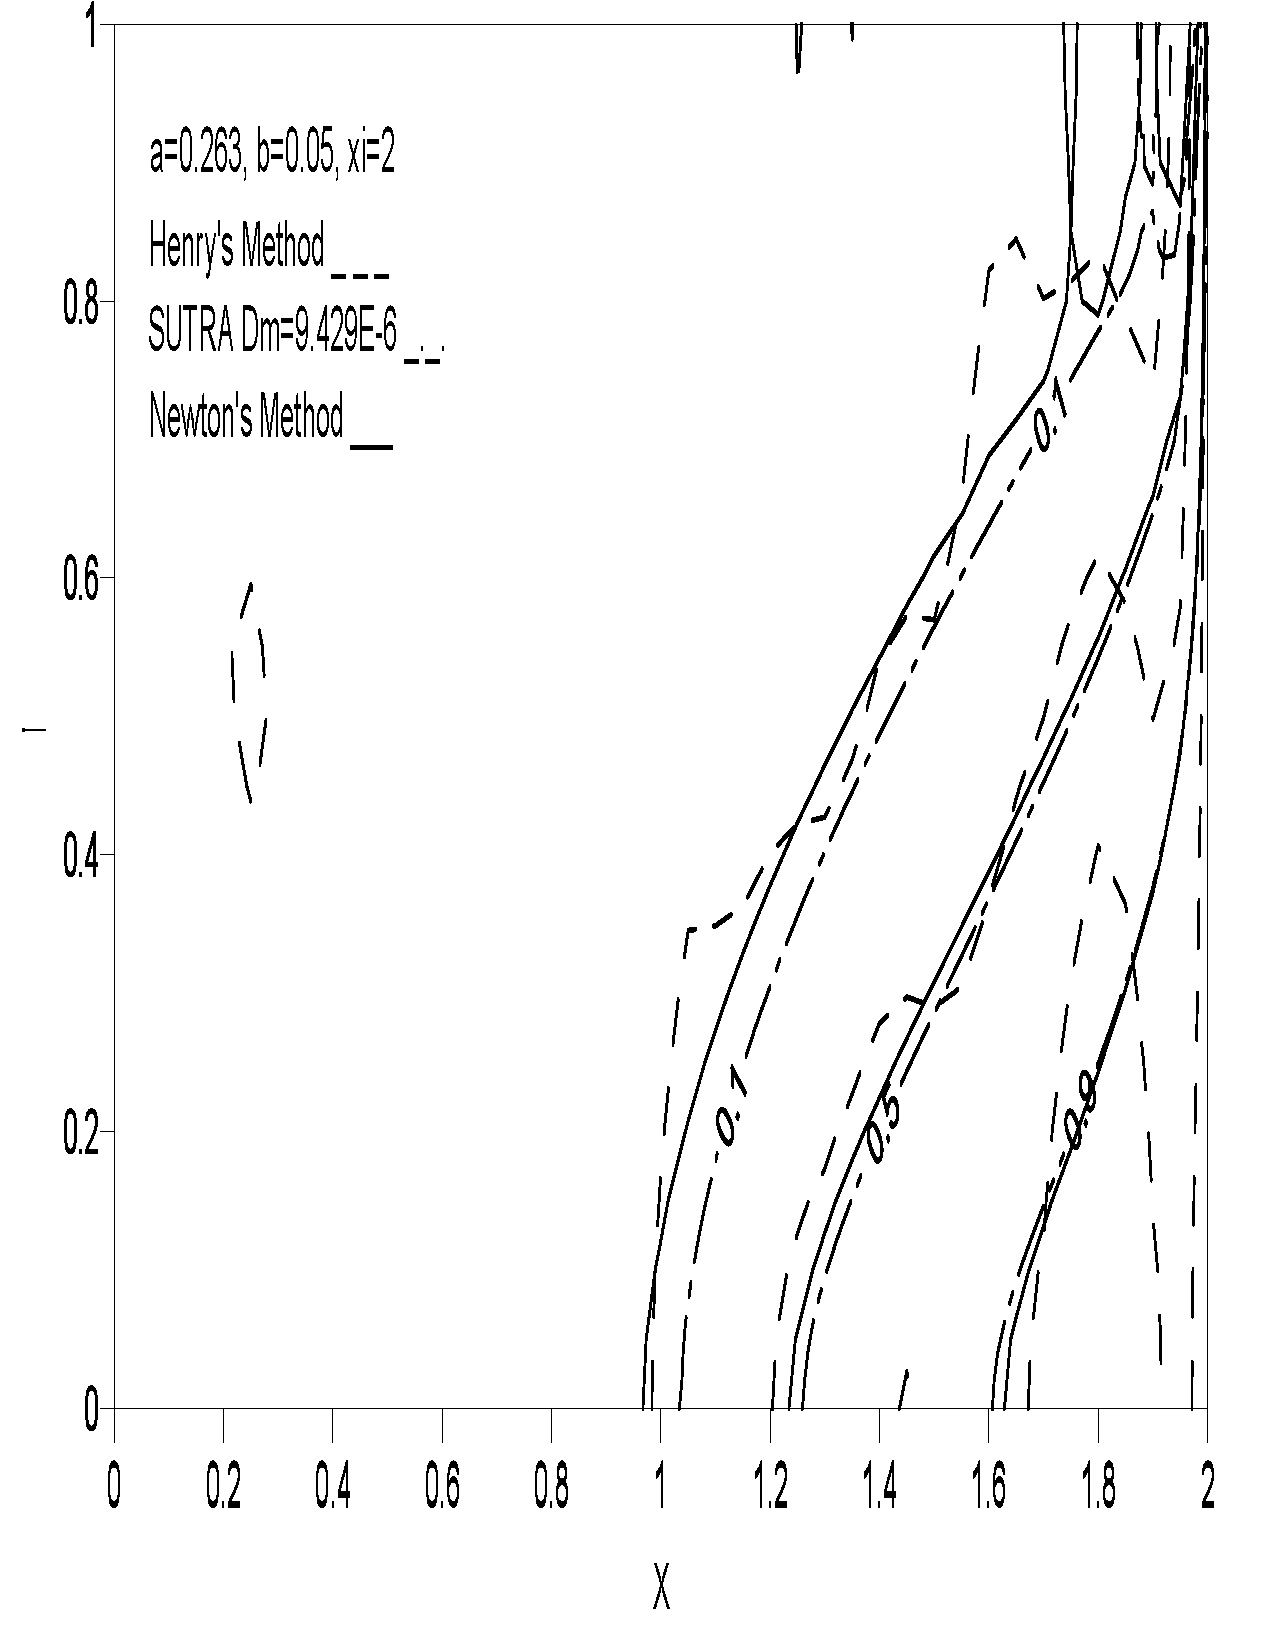
\includegraphics[totalheight=0.45 \textheight,viewport=3mm 4mm 205mm 292mm]
    {image3}
    \caption{Isochlor concentrations fo $a = 0.263 \spbox{and} b =
    0.05$} \label{fig:b5x10-2}
\end{figure}

The third comparison ( \textbf{Figure \ref{fig:b6x10-3}}), for which $b=6\times 10^{-3} $, resulted
in instabilities that created negative and 0.1 isochlors across the entire upper 20\% of the
solution domain for Newton's Method. Similar instabilities can be seen in the SUTRA solution for 231
nodes. One can see in the upper right hand corner the similar pattern that is also present in the
Newton's Method. The resulting 0.1 and 0.5 isochlors no longer match well.  However the 0.9 isochlor
is still very close. But, as one can see the lower values of $b$ create greater and greater
instabilities in the upper 20\% of the solution domain. These instabilities then further degrade the
accuracy of the isochlor contours in the lower 80\% of the solution domain. It is likely that a
larger number of Fourier coefficients could correct these problems, but due to a lack of computing
power and time this was unable to be checked. Henry's Method is not represented in this comparison,
due to the inability of this method to converge for values of $b$ lower than 0.05. It is believed
that the use of more Fourier coefficients would result in better agreement between SUTRA and Henry's
Semi-Analytic Solution.

\begin{figure}[htp]
    \centering
    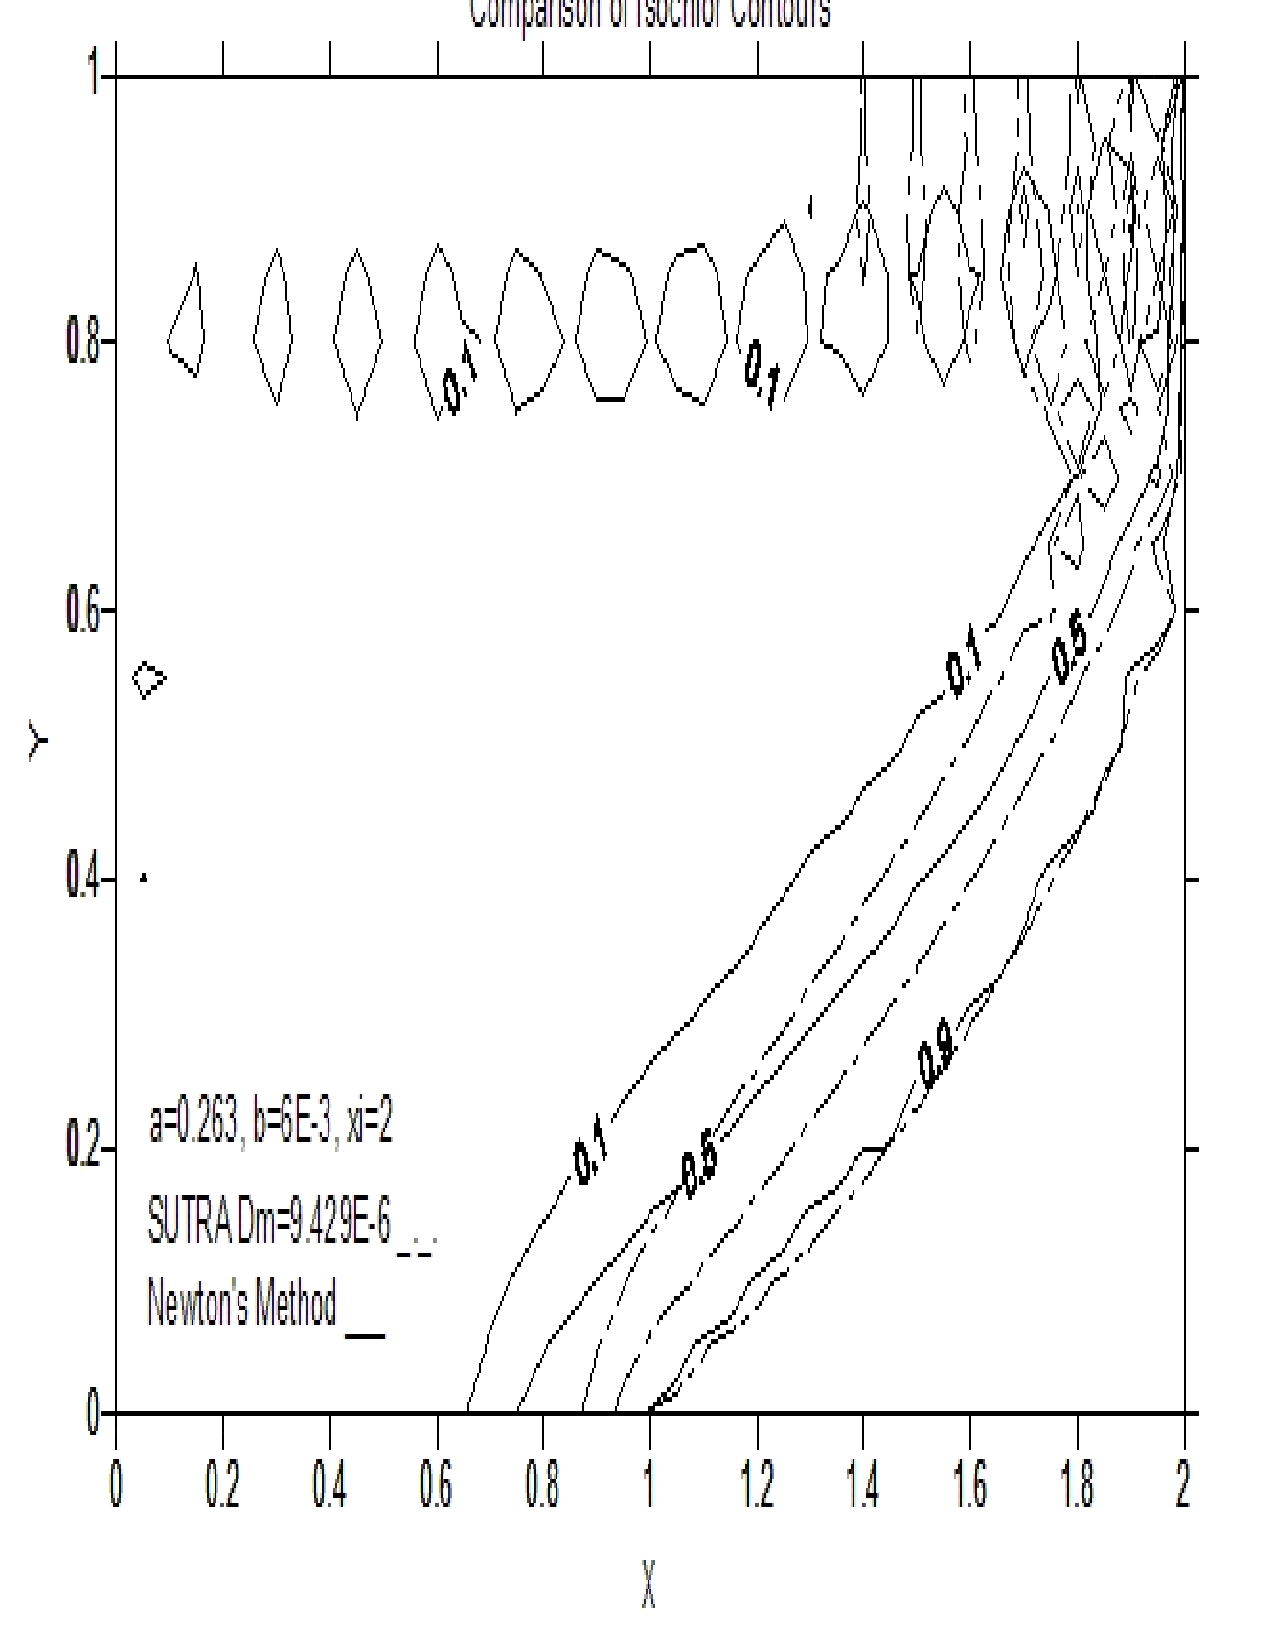
\includegraphics[totalheight=0.45\textheight,viewport=3mm 4mm 205mm 292mm]{image4}
    \caption{Isochlor concentrations for $a = 0.263 \spbox{and} b = 6 \times
    10^{-3}$} \label{fig:b6x10-3}
\end{figure}
